\documentclass[12pt,letterpaper,titlepage]{article}
\usepackage{amsmath}
\usepackage{amsfonts}
\usepackage{amssymb}
\usepackage{caption}
\usepackage{csquotes}
\usepackage[left=1in,right=1in,top=1in,bottom=1in]{geometry}
\usepackage{graphicx}
\usepackage{hyperref}
\usepackage[utf8]{inputenc}

\renewcommand{\refname}{\section{References}}

\title{Thesis Proposal:\\
Selection and Mutation on Correlated\\
Neutral Fitness Landscapes}

\author{George Lesica\\
Department of Computer Science\\
University of Montana\\
Missoula, MT\\
\\
Advisor: Alden Wright}

\begin{document}
\maketitle

\section{Introduction}

\subsection{Biological Neutrality}

\paragraph{}
The theory of neutral evolution was first proposed by Kimura~\cite{Kimura1984}
to explain observed differences between evolution in populations of larger
organisms and evolution at the molecular level. His theory made two
predictions, as laid out by Hughes~\cite{Hughes2007}. First, ``that most
polymorphisms are selectively neutral and are maintained by genetic drift''.
Second, ``that most changes at the molecular level that are fixed over
evolutionary time are selectively neutral and are fixed by drift.''

\paragraph{}
Neutral evolution enables a population to ``explore'' sequence space via
neutral mutation. Neutral mutation itself refers to mutations that have little
or no effect on the fitness of an organism.\footnote{This is not to say that a
neutral mutation has no effect on the phenotype of an organism. Just that
whatever effect it does have does not significantly impact the fitness of the
organism.} In biology, this is the result of the many-to-one relationship
between genotypes and phenotypes~\cite{Newman1998}. While neutral mutations
have no significant effect on fitness, they can pave the way, and can be
necessary conditions, for future beneficial mutations. This type of neutral
mutation is known as a potentiating mutation.

\paragraph{}
A population undergoing neutral evolution is likely to exhibit high genotypic
diversity~\cite{Huynen1996a}. This presents opportunities for the population.
Its members are able to explore the sequence space since selective pressure
does not operate in the context of neutral mutations. As a result, there is a
greater likelihood that some population member will ``discover'' a genotype
that maps to a higher-fitness phenotype, elevating the entire population when,
and if, the mutation reaches fixation.

\subsection{Computational Modeling}

\paragraph{}
In computational modeling we can think of two genotypes that produce the same
phenotype (or which have equal fitness), each of which may be produced by
mutating the other in some small way, as two nodes in a neutral network.

\paragraph{}
Many such networks may exist for a particular genome, each corresponding to a
particular phenotype or fitness level. In some cases, each of these networks
will be small. In other cases, such networks may be expansive and may permeate
the sequence space.

\paragraph{}
A connected component of a network that contains a constant fraction, as
opposed to $O\left(\log n\right)$, of the nodes in the entire network is known
as a giant component. In the case where the neutral network for a given
phenotype (or fitness value) forms a giant component (or comes close) it is
said to be a percolating neutral network.

\subsubsection{Fitness Landscapes}

\paragraph{}
Evolutionary models are composed of a set of genotypes and their corresponding
phenotypes (or simply fitness values).  If we consider an arbitrary model with
only two dimensions, and take fitness as a third dimension, we arrive at a
useful visual metaphor which resembles a topographical map. This motivates the
term ``fitness landscape''. The intuition is that higher ground within the
landscape corresponds to higher fitness.

\paragraph{}
More rigorously, a fitness landscape can be defined as ``a mapping from a
configuration space that is equipped with some notion of adjacency, nearness,
distance or accessibility, into the real numbers.''~\cite{Calcott2008}

\paragraph{}
One important statistical property of a fitness landscape is its ``correlation
structure'', which can be defined simply as ``how similar the fitness values of
one-mutant neighbors in the space are''~\cite{Kauffman1993}. More specifically,
the correlation of a landscape is the expected autocorrelation of a random walk
(see below for a discussion of random and adaptive walks) over
it~\cite{Weinberger1990}. Fitness landscapes are often referred to as
``correlated'' or ``uncorrelated'', depending on the frame of reference.
Visually, an uncorrelated landscape would appear jagged, with some neighboring
points in the space having radically different fitness values.

\paragraph{}
Fitness landscapes are sometimes also referred to as ``smooth'' or ``rugged''.
While these terms do not have rigorous universal definitions, they are
generally defined as landscapes with relatively high autocorrelation and low
autocorrelation, respectively. In other words, on a smooth landscape, the
fitness at a particular point in sequence space can be expected to carry more
information about the fitnesses of its neighbors~\cite{Kauffman1993}.

\subsubsection{Random Walks}

\paragraph{}
We will define a walk through sequence space (or over a fitness landscape,
depending on your point of view) to be a path consisting of a sequence of
genotypes, each of which differs from its neighbors, the genotypes before and
after it in the sequence, by a single mutation.

\paragraph{}
A random walk is a path that is constructed recursively by starting at a
genotype, choosing a random one-mutant neighbor (the choice may be uniformly
random or use some other distribution or algorithm), then repeating the process
for the neighbor.

\subsubsection{Adaptive Walks}

\paragraph{}
An adaptive walk is similar to a random walk. However, instead of choosing
one-mutant neighbors at random, they are chosen with an eye toward improving
the fitness of the selected genotype. The path corresponding to a particular
adaptive walk, then, has the property that each genotype on the path is fitter
than (or at least as fit as) the one that came before it. This process is often
referred to as ``hill-climbing'', which corresponds nicely with the fitness
landscape as a visual metaphor.

\paragraph{}
There are several different methods for choosing the next genotype during an
adaptive walk. Some of the common ones are nicely summarized
in~\cite{Nowak2015}. These include fitness-dependent, where the choice is made
randomly, but fitter genotypes are given preference. Alternately, the choice
can be purely random. A greedy strategy chooses the fittest candidate, and
finally, a reluctant strategy chooses the least fit candidate that is fitter
than the current genotype.

\paragraph{}
If any of the above strategies (which the exception of the reluctant climber)
are allowed to consider mutants that are equally fit in addition to those that
are fitter, the adaptive walk may explore fitness plateaus, or sets of
genotypes with equal fitness.

\paragraph{}
On rugged fitness landscapes, adaptive walks can become ``stuck'' at local
optima because of the constraint that each genotype must be fitter than the one
before it. In fact, this outcome is quite likely. Think of trying to climb
Mount Everest by starting at a random point on the surface of the Earth and
only moving uphill. You would almost certainly end up stuck at the top of some
small hill.

\subsubsection{Neutral Networks}

\paragraph{}
Neutral fitness landscapes are difficult to describe intuitively since all of
their characteristics might also be present in non-neutral landscapes. However,
Crutchfield~\cite{Crutchfield1999} captures the key characteristics. He
describes neutral landscapes as networks of interconnected neutral basins,
see Figure~\ref{fig:crutchfield-basins}. In a way, his description recalls the children's
game ``Chutes and Ladders'', though the mechanics are slightly different.

\begin{figure}
    \centering
    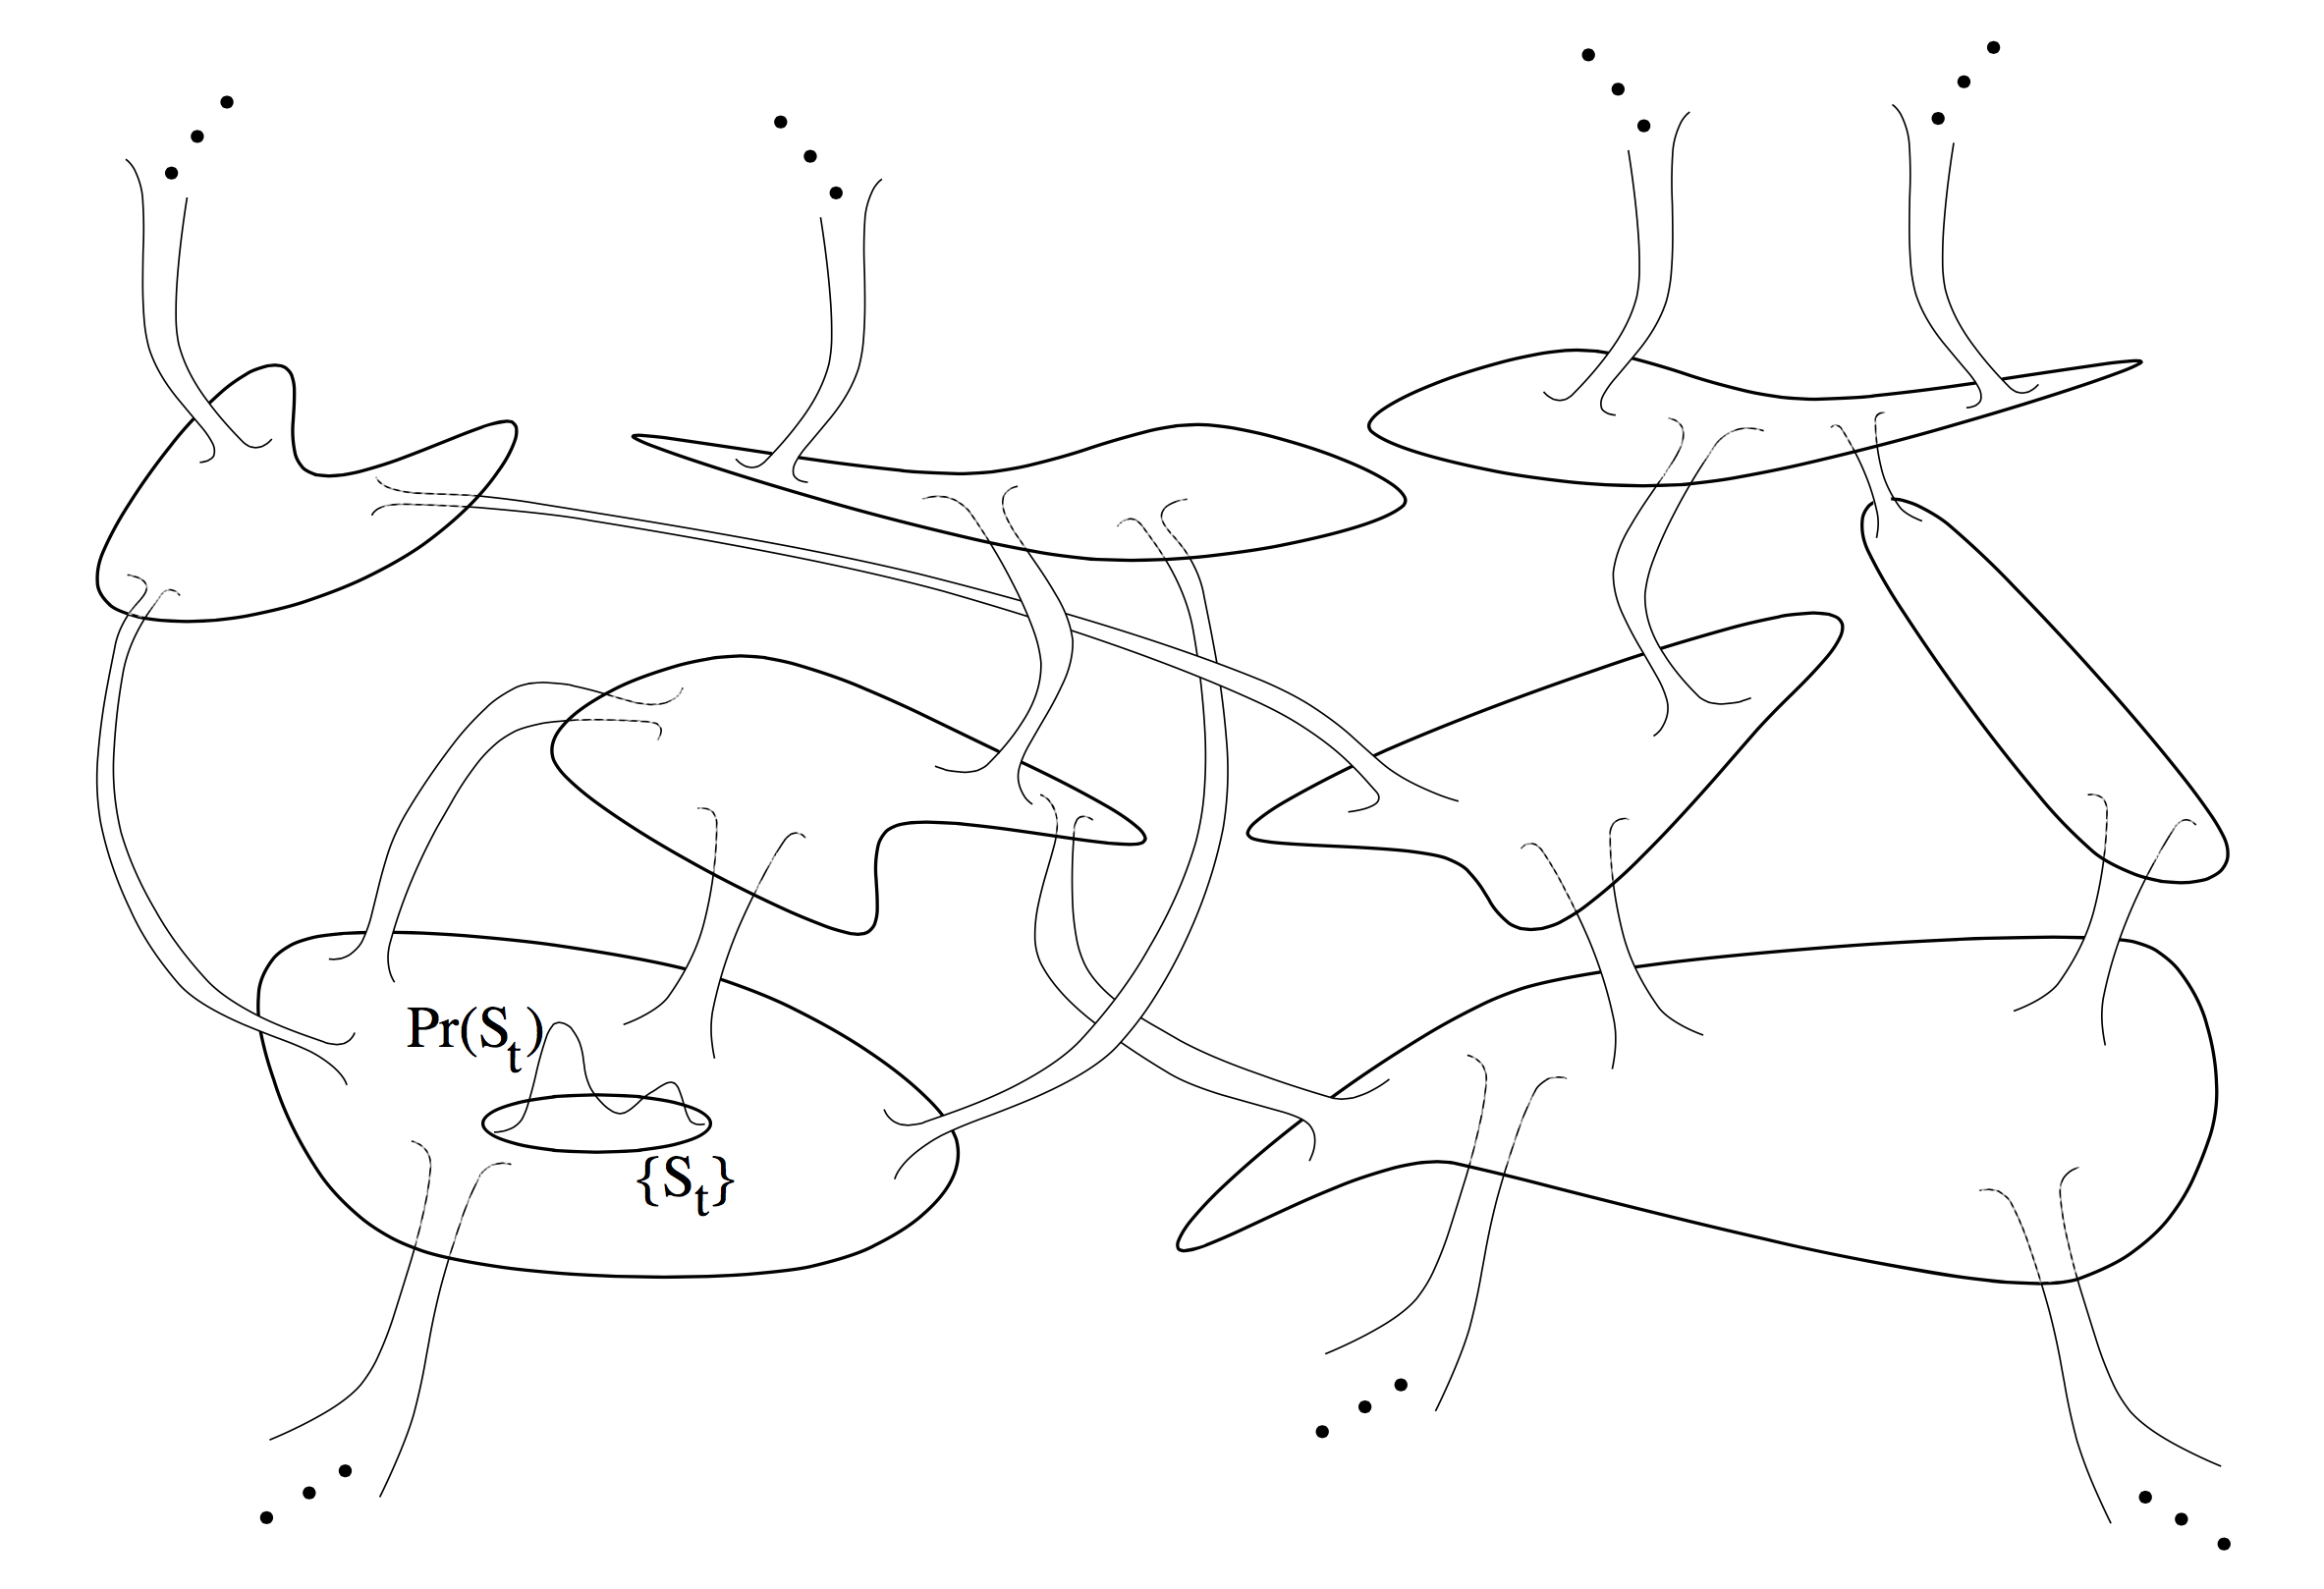
\includegraphics[width=0.8\textwidth]{crutchfield-basins}
    \caption{Crutchfield's neutral basins.}
\label{fig:crutchfield-basins}
\end{figure}

\paragraph{}
Crutchfield describes neutral fitness landscapes as a set of neutral basins,
each with some number of passageways that lead to other basins of higher or
lower fitness (a bit like a multi-level waterfall). A balance between selection
and deleterious mutation prevents the population from falling ``back'' into a
lower fitness basin~\cite{Crutchfield1999}.

\subsubsection{Evolution on Neutral Networks}

\paragraph{}
Adaptive walks on neutral fitness landscapes are likely to result in higher
fitness, as demonstrated by Barnett~\cite{Barnett1998} or, put another way,
populations are less likely to become stuck at local optima~\cite{Newman1998}.

\paragraph{}
We can think of exploring a fitness landscape by following neutral pathways
that may or may not form a percolating (or nearly so) network. Random mutation
drives this process. Eventually (or perhaps frequently), some individual will
mutate off of the neutral network and onto a neutral network with higher
fitness. If this mutation fixes in the population, then the population will
have adapted or evolved.

\paragraph{}
There are two error thresholds that are important in population-based
evolution. The genotypic error threshold is the probability of a single-locus
mutation. When the genotypic error threshold is greater than zero and the
population is evolving on a percolating neutral network the population will
spread out through sequence space. In fact, Huynen et al.\ found that after
roughly 500 generations all of the original sequences had disappeared from the
population.

\paragraph{}
At the same time, however, the phenotypic error threshold, the point beyond
which the dominant phenotype will disappear from the population, is higher that
the genotypic error threshold on neutral networks. This means that while the
original sequences had disappeared after 500 generations, the dominant
phenotype survived until the end of the simulation (1,460 generations).

\section{NK Fitness Landscapes}

\paragraph{}
The NK fitness landscape, developed by Kauffman~\cite{Kauffman1993}, is a
fitness model that features tunable ruggedness. It derives its name from the
fact that an NK landscape is parameterized by two values: $N$, the number of
loci in each genotype, and $K$, the number of loci that are considered
epistatically linked to each locus.

\paragraph{}
The value of $K$ determines how rugged the landscape will be. Higher values
yield greater ruggedness. The special case where $K=0$ yields a landscape with
just a single peak.

\subsection{Construction and Evaluation}

\paragraph{}
An NK landscape is constructed by first choosing values for $N$ and $K$. Then,
for each locus in $N$, $K$ other loci are chosen at random. For each
combination of alleles for those $K+1$ loci (two alleles, 0 and 1, are
typically used for simplicity), a fitness value between zero and one is chosen.

\paragraph{}
Evaluation is done by computing the average fitness across the contributions
from each locus. The contribution for a single locus is computed using the
correct fitness based on the values of the $K+1$ relevant loci and the fitness
table computed when the landscape was created\footnote{In reality, because the
memory required to store such a table grows exponentially with $K$, fitness
values are more commonly generated on-demand. The result, however, is
unchanged.}.

\subsubsection{Example NK Landscape}

\paragraph{}
We will choose $N=3$, and $K=1$ because they yield a simple landscape that
nonetheless exercises all of the model's features. For each of the $N$ loci, in
other words, for each of the slots in a genotype that is part of this model, we
chose 1 other locus to associate with it (Kauffman refers to them as
epistatically linked). Below is an example set of assignments.

\begin{displaymath}
    \left[3,3,1\right]
\end{displaymath}

\paragraph{}
In this particular case, the first locus is linked to the third locus. The
second locus is linked to the third locus as well. Finally, the third locus is
linked to the first locus. Note that nothing is linked to the second locus,
this is perfectly valid.

\paragraph{}
The next step in constructing an NK model, at least conceptually, is to produce
a fitness table for each locus. In this case, $K$ is small, so we can produce a
complete table for each locus. We will assume two alleles and represent them as
0 and 1.

\begin{table}
    \captionsetup{labelformat=empty}
    \parbox{.3\linewidth}{\centering
        \begin{tabular}{l l}
            $\left[0, 0\right]$ & 0.887 \\
            $\left[0, 1\right]$ & 0.411 \\
            $\left[1, 0\right]$ & 0.799 \\
            $\left[1, 1\right]$ & 0.075 \\
        \end{tabular}
        \caption{Table 1}
    }
    \parbox{.3\linewidth}{\centering
        \begin{tabular}{l l}
            $\left[0, 0\right]$ & 0.757 \\
            $\left[0, 1\right]$ & 0.267 \\
            $\left[1, 0\right]$ & 0.355 \\
            $\left[1, 1\right]$ & 0.909 \\
        \end{tabular}
        \caption{Table 2}
    }
    \parbox{.3\linewidth}{\centering
        \begin{tabular}{l l}
            $\left[0, 0\right]$ & 0.830 \\
            $\left[0, 1\right]$ & 0.162 \\
            $\left[1, 0\right]$ & 0.657 \\
            $\left[1, 1\right]$ & 0.211 \\
        \end{tabular}
        \caption{Table 3}
    }
\end{table}

\paragraph{}
We can now evaluate the fitness of any genotype that is valid for our model
(any string of three bits). To do this, we look up a fitness value for each
locus in its table, then average them (to keep the overall fitness value
between 0 and 1). For example, we will evaluate the string
$\left[1,0,1\right]$. First, we look up the fitness for each locus:

\begin{displaymath}
    \left[0.075, 0.267, 0.211\right].
\end{displaymath}

\paragraph{}
Then we average them to yield the fitness for the genotype as a whole: $0.184$.
Note that we used the fourth entry in the first table, because the first locus
is linked to the third locus, and in our example genotype, they are both equal
to 1, so we used the $\left[1, 1\right]$ entry in the first table.

\subsection{Variants}

\paragraph{}
One noteworthy, but perhaps not entirely obvious, implication of the NK design
is that the resultant landscape is almost certainly not neutral, at least
according to a strict definition of the term (see our hypotheses). The
following two variants adapt the general NK landscape to add neutrality.

\subsubsection{NKq Landscapes}

\paragraph{}
The NKq landscape developed by Newman and Engelhardt~\cite{Newman1998} achieves
neutrality using integral fitness values in the tables described above. Instead
of values between zero and one, integers in the interval $\left[0,F-1\right]$
are used, where $F$ is chosen in advance and is often set to 2.

\subsubsection{NKp Landscapes}

\paragraph{}
The NKp landscape, due to Barnett~\cite{Barnett1998}, adds an additional
parameter $p$ which is assigned from the interval $\left[0,1\right]$. When
fitness values are assigned during creation of the landscape, fitness of
exactly 0 is chosen with probability $p$. This means that some loci will have
make no contribution to genotype fitness for certain values of the $K$ loci to
which they are linked. A change at one of these loci will then have no impact
on the fitness of the genotype.

\section{Hypotheses}

\subsection{Real-Valued Fitness Landscapes}

\paragraph{}
It would be useful to have one or more measures of neutrality that would apply
to real-valued fitness landscapes. The NK landscape is generally understood to
be entirely non-neutral. This is a result of the fact that the fitness of a
given point on the landscape is the sum of randomly chosen real values. In
practice, due to the use of floating point values in place of true real values,
two adjacent points on the landscape might have the same fitness value, but it
is incredibly unlikely.

\paragraph{}
However, the biological case for the strict definition of ``neutral'' implied
above is weak. As pointed out by Hughes in~\cite{Hughes2007}:

\begin{displayquote}
An important prediction of the neutral theory is that, when the selection
coefficient in favor of an advantageous mutant or against a deleterious mutant
is less than the reciprocal of twice the effective population size, that mutant
becomes effectively neutral and is not exposed to selection.
\end{displayquote}

\paragraph{}
In the context of an NK landscape, then, neutral neighbors need not have
identical fitness values. The quote above also suggests a definition of
neutrality that might apply comfortably to NK landscapes.

\paragraph{}
Another potential measure of neutrality follows from work by Huynen, Stadler,
and Fontana~\cite{Huynen1996a}. Neutral landscapes exhibit the property that
the genotypic error threshold is lower than the phenotypic error threshold. In
other words, even when the mutation rate is high enough that the population
diffuses away from its initial genotype, the phenotype is still preserved.

\paragraph{}
A significant drawback to this method is that it requires a distinct phenotype,
which the NK model lacks. We may still be able to test it using logic circuits
as a model instead, however.

\paragraph{}
With a definition and measure of neutrality on NK landscapes in-hand, our next
goal will be to determine how changes in the $N$ and $K$ parameters impact
neutrality.

\subsection{Percolation Threshold on NK Landscapes}

\paragraph{}
Gavrilets demonstrated~\cite{Gavrilets1997} that the percolation threshold for
an uncorrelated fitness landscape scales with the inverse of the number of
dimensions under consideration. The percolation threshold is the probability
that a given genotype is part of a particular percolating neutral network
(Gavrilets limited fitness values to ``high'' and ``low'', so the neutral
network in question was the high fitness network). Essentially, the percolation
threshold represents the fraction of the sequence space that must be part of a
neutral network for it to become a percolating network.

\paragraph{}
In other words, as the number of dimensions goes up, it takes a smaller share
of the nodes to create a percolating neutral network. This makes sense because
each additional dimension increases the number of ``routes'' between two
points. This is really quite intuitive for low dimensions. For example, imagine
a video game like Super Mario Brothers in which the character moves in two
dimensions. Many a child has observed in frustration (or perhaps annoyance)
that most of the puzzles in such games would be trivial if only a third
dimension were available to allow greater freedom of movement.

\paragraph{}
We hypothesize that the relationship identified by Gavrilets holds for NK
landscapes as well, using the measure of neutrality we intend to develop.

\section{Methods}

\paragraph{}
To facilitate testing our hypotheses, we intend to create two pieces of
reusable software, both of which will be released as open source software.

\subsection{NK.jl Library}

\paragraph{}
We have opted to generalize our NK landscape
implementation\footnote{\url{https://github.com/glesica/NK.jl}} so that it may
be used by others in the future. We will provide it as a separate package under
a permissive license that will hopefully allow future work and improvement.  We
will use this library for our own experiments in addition to contributing it to
the community as open source software.

\paragraph{}
We intend to implement several NK variants including NKq and NKp neutral
landscapes. We will also provide implementations of several common techniques
such as adaptive walks and proportional selection from a population.

\subsection{CGP.jl Library}

\paragraph{}
Cartesian Genetic Programming (CGP) eschews the tree structures more commonly
associated with genetic programming in favor of a grid (hence ``Cartesian'') of
functions that can take as their inputs the outputs from any preceding
functions. Our CGP library\footnote{\url{https://github.com/glesica/CGP.jl}}
attempts to combine computation performance with ease-of-use.

\section{Experiments}

\section{Analysis}

\bibliographystyle{acm}
\bibliography{fitness}{}
\end{document}
